\documentclass[10pt]{beamer}
\usepackage{tikz}
\usepackage{kotex}
\usepackage{amsmath,amsfonts,amssymb,mathrsfs,mathtools,adjustbox,float,graphicx}
\usepackage{dtk-logos}
\usepackage{xcolor}
\usepackage{setspace}
\usepackage{minted}
\usepackage{expl3}
\usepackage{xparse}
\usepackage{enumitem}
\usepackage{forloop}
\usefonttheme[onlymath]{serif}

\AtBeginSection[]{
  \begin{frame}
  \vfill
  \centering
  \begin{beamercolorbox}[sep=8pt,center,shadow=false,rounded=true]{title}
    \usebeamerfont{title}\insertsectionhead\par%
  \end{beamercolorbox}
  \vfill
  \end{frame}
}

\setlist[itemize,1]{label=\usebeamerfont*{itemize item}%
  \usebeamercolor[fg]{itemize item}
  \usebeamertemplate{itemize item}}
\setlist[itemize,2]{label=\usebeamerfont*{itemize subitem}%
  \usebeamercolor[fg]{itemize subitem}
  \usebeamertemplate{itemize subitem}}
\setlist[itemize,3]{label=\usebeamerfont*{itemize subsubitem}%
  \usebeamercolor[fg]{itemize subsubitem}
  \usebeamertemplate{itemize subsubitem}}
\AtBeginEnvironment{minted}{\singlespacing\fontsize{9}{12}\selectfont}
\newminted{latex}{breaklines=true,breaksymbolleft={}}
\usemintedstyle{manni}
\setminted{bgcolor=white!95!black}
\setmintedinline{fontsize=\small}

\setstretch{1.3}
\usetikzlibrary{shapes.geometric}

\makeatother
\setbeamertemplate{footline}
{
	\leavevmode%
	\hbox{%
		\begin{beamercolorbox}[wd=.3\paperwidth,ht=2.25ex,dp=1ex,center]{author in head/foot}%
			\usebeamerfont{author in head/foot}\insertshortauthor
		\end{beamercolorbox}%
		\begin{beamercolorbox}[wd=.6\paperwidth,ht=2.25ex,dp=1ex,center]{title in head/foot}%
			\usebeamerfont{title in head/foot}\insertshorttitle
		\end{beamercolorbox}%
		\begin{beamercolorbox}[wd=.1\paperwidth,ht=2.25ex,dp=1ex,center]{date in head/foot}%
			\insertframenumber{} / \inserttotalframenumber\hspace*{1ex}
	\end{beamercolorbox}}%
	\vskip0pt%
}

\makeatletter
\setbeamertemplate{navigation symbols}{}

\def\setfont{
    \ifPDFTeX
        \PackageError{MathLetter}{%
            PDFTeX is not allowed to set fonts!
        }{%
            Use another engine, such as XeLaTeX or LuaLaTeX.
        }
    \fi
    \setsansfont{Noto Sans CJK KR}[Scale=0.90,ItalicFont={*},ItalicFeatures={FakeSlant=.167}]
    \setmainhangulfont[Scale=0.94]{Noto Serif CJK KR}
    \setmainhangulfont
        [ItalicFont={*},ItalicFeatures={FakeSlant=.167}]
        {Noto Serif CJK KR}
    \setsanshangulfont[Scale=0.94]{Noto Sans CJK KR}
    \setsanshangulfont
        [ItalicFont={*},ItalicFeatures={FakeSlant=.167}]
        {Noto Sans CJK KR}[Scale=0.94]
    \setmonohangulfont{Noto Sans Mono CJK KR}
    \setmonohangulfont
        [ItalicFont={*},ItalicFeatures={FakeSlant=.167}]
        {Noto Sans Mono CJK KR}
}

\setfont


% setting some colors for the theme
\setbeamercolor{palette primary}{fg=black,bg=white}
\setbeamercolor{palette secondary}{fg=black,bg=white}
\setbeamercolor{structure}{fg=black,bg=white}
\setbeamercolor{title in head/foot}{fg=black,bg=white}
\setbeamercolor{date in head/foot}{fg=black,bg=white}



% definition of the title page template
\defbeamertemplate*{title page}{mytheme}[1][]
{%
  \begin{tikzpicture}[remember picture,overlay]
  \filldraw[white]
    (current page.north west) --
    (current page.north east) --
    ([xshift=0cm,yshift=-2cm]current page.north east)  --
    ([xshift=0cm,yshift=-2cm]current page.north west) -- cycle
    ;
   \node[opacity=0.4] at (current page.center) 
    {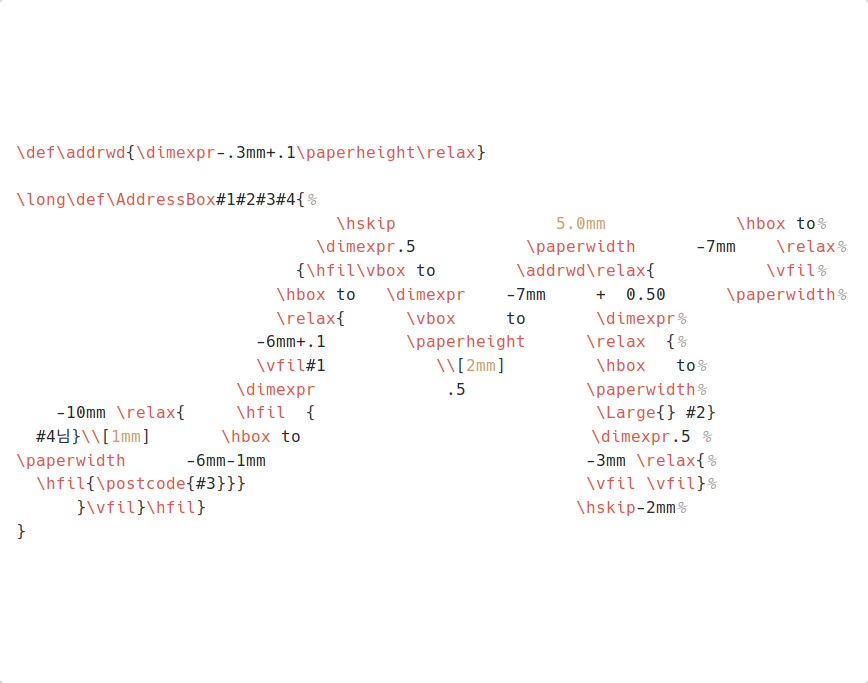
\includegraphics[scale=0.4]{msquare}};
  \node[text=black,anchor=center,font=\sffamily\LARGE,text width=\paperwidth] 
  at (current page.center)
  (title)
  {\begin{center}\inserttitle\end{center}};
    
    \node[text=black,anchor=south west,font=\sffamily\small,text width=.6\paperwidth] 
  at ([xshift=-100pt,yshift=-1.5cm]current page.center)
  (institute)
  {\raggedright\insertinstitute};
   
  \node[anchor=west]
  at ([xshift=-100pt,yshift=1cm]current page.south east)
  {};
  \node[text=black,font=\large\sffamily,anchor=south west]
  at ([xshift=30pt,yshift=0.5cm]current page.south west)
  (date)
  {\insertdate};
  \node[text=black,font=\large\sffamily,anchor=south west]
  at ([yshift=5pt]date.north west)
  (author)
  {\insertauthor};
  \end{tikzpicture}%
}

% remove navigation symbols
\setbeamertemplate{navigation symbols}{}

\definecolor{color0}{HTML}{FEABB7}
\definecolor{color1}{HTML}{9797B9}
\definecolor{color2}{HTML}{4B7AA3}

% definition of the symbols used in itemize
\newcommand\mysymbol{%
  
\begin{tikzpicture}[xscale=0.85]
    \draw (1.75ex,0) node[star, star points=5, star point ratio=2.25, inner sep=1.3pt,anchor=outer point 3,fill=color0] {};          
  \end{tikzpicture}%
}
\newcommand\mysymboli{%
  
\begin{tikzpicture}[xscale=0.85]
    \draw (1.75ex,0) node[star, star points=5, star point ratio=2.25, inner sep=1.3pt,anchor=outer point 3,fill=color1] {};          
  \end{tikzpicture}%
}
\newcommand\mysymbolii{%
  
\begin{tikzpicture}[xscale=0.85]
    \draw (1.75ex,0) node[star, star points=5, star point ratio=2.25, inner sep=1.3pt,anchor=outer point 3,fill=color2] {};          
  \end{tikzpicture}%
}

% definition of the itemize templates
\defbeamertemplate*{itemize item}{mysymbol}{\small\raise-0.5pt\hbox{\mysymbol}}
\defbeamertemplate*{itemize subitem}{mysymbol}{\footnotesize\raise-0.5pt\hbox{\mysymboli}}
\defbeamertemplate*{itemize subsubitem}{mysymbol}{\footnotesize\raise-0.5pt\hbox{\mysymbolii}}

\makeatletter
\newlength{\raising}
\newcommand{\MSquare}[1][1]{\colorlet{currentcolor}{.}\setlength{\raising}{-1pt*\ratio{\f@size pt}{5.5pt}}\edef\xscaleFactor{(0.026 * \f@size)}\edef\yscaleFactor{(-1 * \xscaleFactor)}%
\raisebox{\raising}{\begin{tikzpicture}[y=0.80pt, x=0.80pt, yscale=\yscaleFactor, xscale=\xscaleFactor, inner sep=0pt, outer sep=0pt]
\begin{scope}[shift={(0,-229.26665)},xscale=#1,yscale=#1]
\path[line width=0.065pt,fill=currentcolor] (60.5716,281.9345) -- (61.5507,279.9761) .. controls
(62.2579,278.6162) and (62.9515,277.1474) .. (63.6315,275.5699) .. controls
(64.3114,273.9923) and (65.0458,272.1972) .. (65.8346,270.1845) .. controls
(66.6233,268.1717) and (67.2353,266.6758) .. (67.6705,265.6966) .. controls
(71.0976,257.4825) and (74.0623,251.6891) .. (76.5646,248.3165) .. controls
(78.0877,246.1949) and (79.6109,244.5902) .. (81.1340,243.5023) .. controls
(83.1467,242.0335) and (84.3163,242.4959) .. (84.6427,244.8894) .. controls
(84.7515,245.7054) and (84.6971,247.2557) .. (84.4795,249.5404) .. controls
(84.2619,251.3356) and (83.9763,253.2259) .. (83.6227,255.2114) .. controls
(83.2691,257.1969) and (82.8204,259.4409) .. (82.2764,261.9432) .. controls
(81.7324,264.4455) and (81.3516,266.3222) .. (81.1340,267.5734) .. controls
(79.9373,273.5571) and (79.7469,278.9969) .. (80.5628,283.8928) .. controls
(80.9980,287.1567) and (82.1132,289.7949) .. (83.9083,291.8077) .. controls
(84.2347,292.1341) and (84.4523,292.3789) .. (84.5611,292.5420) .. controls
(84.9963,293.1948) and (85.0235,293.7932) .. (84.6427,294.3372) .. controls
(84.2075,294.8268) and (83.6363,294.8812) .. (82.9291,294.5004) .. controls
(82.2764,294.1740) and (81.7596,293.7388) .. (81.3788,293.1948) .. controls
(78.7133,289.6590) and (76.9454,285.4431) .. (76.0750,280.5473) .. controls
(75.4766,276.9026) and (75.5038,272.5508) .. (76.1566,267.4918) .. controls
(76.3742,265.8598) and (76.7550,263.5615) .. (77.2989,260.5968) .. controls
(77.8429,257.6321) and (78.2237,255.4698) .. (78.4413,254.1099) .. controls
(78.7133,252.1515) and (78.7133,250.4108) .. (78.4413,248.8877) .. controls
(78.2237,249.2140) and (77.9245,249.7308) .. (77.5437,250.4380) .. controls
(77.1629,251.1452) and (76.8910,251.6619) .. (76.7278,251.9883) .. controls
(74.3343,256.2314) and (71.6416,261.9704) .. (68.6497,269.2053) .. controls
(65.9842,275.5155) and (64.3794,279.1601) .. (63.8354,280.1393) .. controls
(61.9859,283.5120) and (60.0820,285.7967) .. (58.1236,286.9935) .. controls
(57.5797,287.3198) and (57.1717,287.1838) .. (56.8997,286.5855) .. controls
(55.3765,283.0496) and (54.7238,279.5681) .. (54.9414,276.1411) .. controls
(54.9958,275.1619) and (55.1454,273.7611) .. (55.3901,271.9388) .. controls
(55.6349,270.1165) and (55.7845,268.8517) .. (55.8389,268.1446) .. controls
(55.9477,266.9478) and (56.1925,264.9351) .. (56.5733,262.1064) .. controls
(56.9541,259.2777) and (57.1989,257.1018) .. (57.3077,255.5786) .. controls
(57.5797,252.6955) and (57.7157,250.1116) .. (57.7157,247.8269) --
(57.7157,247.0109) -- (57.4709,247.0109) .. controls (55.4037,250.3836) and
(53.6358,254.1371) .. (52.1671,258.2713) .. controls (49.7736,265.1799) and
(47.8968,269.9941) .. (46.5369,272.7140) .. controls (43.9258,277.9362) and
(40.7163,281.6896) .. (36.9084,283.9744) .. controls (33.8077,285.8783) and
(30.3535,287.0478) .. (26.5456,287.4830) .. controls (23.4993,287.8094) and
(20.6434,287.9454) .. (17.9779,287.8910) .. controls (12.4837,287.6734) and
(8.4039,287.1294) .. (5.7384,286.2591) .. controls (4.7592,285.9327) and
(3.7800,285.4703) .. (2.8009,284.8719) .. controls (0.5162,283.4576) and
(0.1626,281.6624) .. (1.7401,279.4865) .. controls (2.7737,278.0722) and
(4.4872,276.6578) .. (6.8807,275.2435) .. controls (10.6886,273.0132) and
(15.5028,271.0004) .. (21.3234,269.2053) .. controls (27.6336,267.3014) and
(33.9981,265.8326) .. (40.4171,264.7991) .. controls (41.5051,264.5815) and
(42.3754,264.4999) .. (43.0282,264.5543) .. controls (43.5178,264.6631) and
(43.8714,264.8807) .. (44.0890,265.2071) .. controls (44.1978,265.5334) and
(44.0618,265.8870) .. (43.6810,266.2678) .. controls (43.1370,266.8662) and
(41.9946,267.5734) .. (40.2539,268.3893) .. controls (37.2620,269.5861) and
(32.1214,271.0276) .. (24.8321,272.7140) .. controls (17.8147,274.3459) and
(13.1909,275.5699) .. (10.9606,276.3858) .. controls (7.9143,277.5826) and
(5.7384,278.7793) .. (4.4328,279.9761) .. controls (3.5625,280.6833) and
(3.1817,281.2545) .. (3.2905,281.6896) .. controls (3.3449,281.9616) and
(3.4673,282.1384) .. (3.6577,282.2200) .. controls (3.8480,282.3016) and
(4.1200,282.3696) .. (4.4736,282.4240) .. controls (4.8272,282.4784) and
(5.0312,282.5056) .. (5.0856,282.5056) .. controls (5.6840,282.6144) and
(8.5399,282.8048) .. (13.6533,283.0768) .. controls (16.6996,283.1856) and
(20.3442,283.1584) .. (24.5873,282.9953) .. controls (29.1567,282.7777) and
(32.6654,282.1521) .. (35.1133,281.1186) .. controls (38.5948,279.6498) and
(41.4235,276.9299) .. (43.5994,272.9589) .. controls (44.6329,271.1637) and
(46.1017,267.4919) .. (48.0056,261.9433) .. controls (50.0727,256.0683) and
(51.7319,252.0428) .. (52.9830,249.8669) .. controls (54.6150,247.0382) and
(56.4101,244.7535) .. (58.3684,243.0128) .. controls (58.9668,242.4688) and
(59.6468,242.0336) .. (60.4084,241.7072) .. controls (61.5507,241.2720) and
(62.2851,241.5984) .. (62.6115,242.6864) .. controls (62.8835,243.6111) and
(63.0739,244.7263) .. (63.1827,246.0319) .. controls (63.3459,250.3837) and
(62.9923,255.5243) .. (62.1219,261.4537) .. controls (60.9795,269.6134) and
(60.3540,274.2916) .. (60.2452,275.4884) .. controls (60.0820,277.6099) and
(60.1092,279.5954) .. (60.3268,281.4450) .. controls (60.2724,281.6081) and
(60.3540,281.7713) .. (60.5716,281.9345) -- cycle(93.0472,250.7644) --
(99.0038,250.7644) .. controls (99.6565,250.7100) and (100.0917,250.8324) ..
(100.3093,251.1316) .. controls (100.5269,251.4308) and (100.6357,251.9067) ..
(100.6357,252.5595) .. controls (100.6357,252.9947) and (100.6085,253.3347) ..
(100.5541,253.5795) .. controls (100.4997,253.8243) and (100.3501,254.0283) ..
(100.1053,254.1915) .. controls (99.8605,254.3547) and (99.4933,254.4363) ..
(99.0038,254.4363) .. controls (95.6311,254.3819) and (92.2584,254.3819) ..
(88.8857,254.4363) .. controls (87.7978,254.4363) and (87.3626,253.9467) ..
(87.5802,252.9675) .. controls (87.9066,251.0092) and (88.8857,249.2412) ..
(90.5177,247.6637) .. controls (91.0073,247.2829) and (91.7280,246.6845) ..
(92.6800,245.8686) .. controls (93.6320,245.0526) and (94.3527,244.4270) ..
(94.8423,243.9918) .. controls (95.9847,243.0671) and (96.4743,241.8703) ..
(96.3111,240.4016) .. controls (96.0935,239.0416) and (95.4679,238.3072) ..
(94.4343,238.1985) .. controls (93.1288,238.0353) and (92.2584,238.6336) ..
(91.8232,239.9936) .. controls (91.7688,240.1024) and (91.7417,240.3064) ..
(91.7417,240.6056) .. controls (91.7417,240.9048) and (91.7009,241.1495) ..
(91.6193,241.3399) .. controls (91.5377,241.5303) and (91.3881,241.6527) ..
(91.1705,241.7071) .. controls (90.5721,241.9247) and (89.6473,241.9247) ..
(88.3962,241.7071) .. controls (87.8522,241.6527) and (87.6618,241.2719) ..
(87.8250,240.5648) .. controls (87.9338,239.3136) and (88.3554,238.1440) ..
(89.0897,237.0561) .. controls (89.8241,235.9681) and (90.7081,235.2609) ..
(91.7417,234.9346) .. controls (94.6791,234.0642) and (97.0726,234.7170) ..
(98.9222,236.8929) .. controls (100.7173,238.9600) and (101.0437,241.2447) ..
(99.9013,243.7470) .. controls (99.3574,244.9438) and (98.5414,245.9502) ..
(97.4534,246.7661) .. controls (96.9639,247.0925) and (95.4679,248.3165) ..
(92.9656,250.4380) .. controls (92.9656,250.5468) and (92.9928,250.6556) ..
(93.0472,250.7644) -- cycle;
\end{scope}
\end{tikzpicture}}}
\makeatother


\title[]{\bf2019 편집부 \LaTeX\ 세미나}
\author{}
\date{}

\institute{}

\begin{document}

\begin{frame}[plain]
  \maketitle
\end{frame}

\section{Introduction}

\begin{frame}
  \frametitle{\LaTeX\ 설치하기}
  \framesubtitle{}
  \begin{itemize}
    \item \TeX은 여러 가지 배포판이 있습니다.
    \item \TeX\,Live 배포판 설치하기 (가장 쉬운 방법)
    \begin{itemize}
      \item \url{https://www.tug.org/texlive/}에 방문하여 설치
      \item \texttt{texlive-full}을 받으면 정신건강에 매우 편하지만, 약 \textbf{4.9 GB}를 차지합니다.
      \item \texttt{texlive-basic}을 받으면 초기 용량을 \textbf{64 MB}까지 줄일 수 있지만, 필요한 패키지를 일일이 설치해야 합니다.
    \end{itemize}
    \item MikTeX (Windows) {\small(\url{https://miktex.org/})}
    \item TnXTeX {\small(\url{http://wiki.ktug.org/wiki/wiki.php/TnXTeX})}
    \item TinyTeX {\small(\url{https://yihui.name/tinytex/})}
  \end{itemize}
  \vskip.5em
  
  MikTeX은 \TeX\,Live 기반 배포판과 설정 방법이 달라 추천드리지 않습니다.
  
  \end{frame}
  
  \begin{frame}
  \frametitle{\TeX\,Live 패키지 설치하기 (스킵 가능)}
  \framesubtitle{}
  \begin{itemize}
    \item \texttt{texlive-full}이 아닌 더 적은 패키지를 포함하고 있는 버전을 받으셨다면, 추가로 설치해야 하는 패키지들이 있을 수 있습니다.
    \item 문서를 작성하다가 \texttt{File `\string~\string~\string~.sty' not found.}라는 에러 메시지가 발생하면, 다음 명령어를 터미널 (혹은 cmd)에 입력해 주세요.
    \begin{itemize}
      \item \texttt{tlmgr search --global --file "/패키지\_이름.sty"}를 입력하면
      \item `\texttt{패키지\_묶음\_이름:\quad texmf-dist/.../패키지\_이름.sty}'라는 문구를 볼 수 있고,
      \item \texttt{tlmgr install 패키지\_묶음\_이름}을 치면 설치됩니다.
    \end{itemize}
    \item 다운로드 받은 \texttt{sty} 파일을 설치하고 싶다면, \url{https://github.com/msquare-kaist/mathletter-package/blob/master/documents/manual.pdf}를 참조해 주세요.
  \end{itemize}
  
  \end{frame}
  
  
  \begin{frame}
    \frametitle{\TeX이란?}
    \framesubtitle{}
    \begin{itemize}
      \item \TeX: Donald Knuth가 개발한 문서 조판 도구
      \item \LaTeX: Leslie B. Lamport가 개발한 \TeX의 확장\,(매크로 모음)
      \begin{itemize}
        \item \LaTeXe: 가장 많이 쓰이는 \LaTeX\ 버전
        \item \LaTeX\,3: 현재 개발 중인 \LaTeX\ 버전
      \end{itemize}
      \item 이외에도 \ConTeXt이라는 확장이 있습니다.
      \item Overleaf: 가장 유명한 온라인 \LaTeX\ 동시 편집 서비스 (\url{https://overleaf.com})
    \end{itemize}
  \end{frame}
  
  \makeatletter
  \NewDocumentCommand\newterm{m o}{%
    \textbf{#1}%
    \IfNoValueF{#2}{\kern1pt{\small(#2)}\expandafter\ltx@ifnextchar@nospace{ }{}{\kern1pt}}%
  }
  \makeatother
  
  \begin{frame}[fragile]
    \frametitle{Token}
    \framesubtitle{}
    \begin{itemize}
      \item \TeX\ 문서는 토큰들로 이루어져 있으며, \TeX\ 엔진이 각 토큰을 \newterm{전개}[expand]하면서 실행됩니다.
      \item \newterm{매크로}[macro] 또는 \newterm{정의}[definition]란 기본적으로 정의되어 있는 토큰들{\,\small(primitives)\,}을 이용하여 정의된 토큰들을 말합니다.
      \item 매크로는 보통 \mintinline[escapeinside=||]{latex}{\macro}와 같이 백슬래시로 시작하고 알파벳이 뒤에 따라 옵니다.
      \item 한 글자짜리 매크로는 알파벳이 아니어도 올 수 있습니다. \mintinline[escapeinside=||]{latex}{\ }, \mintinline[escapeinside=||]{latex}{\#}, ...
    \end{itemize}
  \end{frame}
  
  \begin{frame}[fragile]
    \frametitle{문서 구조}
    \framesubtitle{}
    \begin{itemize}
      \item \mintinline[escapeinside=||]{latex}{\documentclass[a4paper,11pt]{article}} 문서의 논리적 구조를 지정합니다.
      \begin{itemize}
        \item \texttt{book}, \texttt{report}, \texttt{memoir} 등의 class가 있습니다.
      \end{itemize}
      \item \mintinline[escapeinside=||]{latex}{\usepackage{amsmath}} 미리 정의된 매크로를 \newterm{패키지}에서 가져옵니다.
      \begin{itemize}
        \item 사실은 \mintinline[escapeinside=||]{latex}{\usepackage}는 \mintinline[escapeinside=||]{latex}{\RequirePackage}로 정의됩니다.
      \end{itemize}
      \item \mintinline[escapeinside=||]{latex}{\title{...}}, \mintinline[escapeinside=||]{latex}{\author{...}}, \mintinline[escapeinside=||]{latex}{\date{...}}
      \item \mintinline[escapeinside=||]{latex}{\begin{document}} 문서를 시작합니다.
      \item \mintinline[escapeinside=||]{latex}{\maketitle} 제목, 저자, 날짜를 출력합니다.
      \item \mintinline[escapeinside=||]{latex}{% 주석입니다} 퍼센트 기호 뒤는 무시됩니다.
      \item \mintinline[escapeinside=||]{latex}{\end{document}} 문서를 끝냅니다.
    \end{itemize}
  \end{frame}
  
  \begin{frame}[fragile]
    \frametitle{Sample Document}
    \framesubtitle{따라만 하세요 따라만 하세요}
    \begin{minted}{latex}
\documentclass[a4paper,10pt]{article}
\usepackage{amsmath}
\usepackage{kotex}
\title{제목}

\begin{document}
\maketitle

안녕하세요? \LaTeX을 배우면 좋은 일이 있을 거예요. % 아닐 수도..

\makeatletter
당신이 입력했던 제목입니다: \@title.
\makeatother
\end{document}
  \end{minted}
  \end{frame}
  
  \begin{frame}[fragile]
    \frametitle{글씨체}
    \framesubtitle{일반 텍스트의 글씨체}
    \begin{itemize}
      \item \mintinline[escapeinside=||]{latex}{{\normalfont 기본 폰트}} {\normalfont 기본 폰트}
      \item \mintinline[escapeinside=||]{latex}{\textbf{굵게}}, \mintinline[escapeinside=||]{latex}{{\bfseries 굵게}} \textbf{굵게}
      \item \mintinline[escapeinside=||]{latex}{\textit{이탤릭}}, \mintinline[escapeinside=||]{latex}{{\itshape 이탤릭}} \textit{이탤릭}
      \begin{itemize}
        \item \mintinline[escapeinside=||]{latex}{\textit}는 그 다음에 똑바로 선 글자가 왔을 때 간격 보정을 해줍니다.
        \item \mintinline[escapeinside=||]{latex}{\textit{(이탤)}릭}, \mintinline[escapeinside=||]{latex}{{\itshape (이탤)}릭}
        \item 
\includegraphics[width=0.09\textwidth]{italic}
      \end{itemize}
      \item \mintinline[escapeinside=||]{latex}{\textrm{명조}}, \mintinline[escapeinside=||]{latex}{{\rmfamily 명조}} \textrm{명조}
      \item \mintinline[escapeinside=||]{latex}{\textsf{돋움}}, \mintinline[escapeinside=||]{latex}{{\sffamily 돋움}} \textsf{돋움}
      \item \mintinline[escapeinside=||]{latex}{\textsl{기울임}}, \mintinline[escapeinside=||]{latex}{{\slshape 기울임}} \textsl{기울임}
      \item \mintinline[escapeinside=||]{latex}{\textsc{SmallCaps}}, \mintinline[escapeinside=||]{latex}{{\scshape SmallCaps}} \textsc{SmallCaps}
      \item \mintinline[escapeinside=||]{latex}{\texttt{typewriter}}, \mintinline[escapeinside=||]{latex}{{\ttfamily typewriter}} \texttt{typewriter}
    \end{itemize}
  \end{frame}
  
  \begin{frame}[fragile]
    \frametitle{글씨체}
    \framesubtitle{수식 모드의 글씨체}
    \begin{itemize}
      \item \mintinline[escapeinside=||]{latex}{\mathbf{Bold}} $\mathbf{Bold}$
      \item \mintinline[escapeinside=||]{latex}{\boldsymbol{\alpha}} $\boldsymbol{\alpha}$ (알파벳이나 숫자가 아닌 기호를 굵게)
      \item \mintinline[escapeinside=||]{latex}{\mathit{italic}} $\mathit{italic}$
      \item \mintinline[escapeinside=||]{latex}{\mathrm{Roman}} $\mathrm{Roman}$
      \item \mintinline[escapeinside=||]{latex}{\mathsf{Sans-serif}} $\mathsf{Sans-serif}$
      \item \mintinline[escapeinside=||]{latex}{\mathbb{BLACK}} $\mathbb{BLACK}$
      \item \mintinline[escapeinside=||]{latex}{\mathcal{CALI}} $\mathcal{CALI}$
      \item \mintinline[escapeinside=||]{latex}{\mathscr{SCRIPT}} $\mathscr{SCRIPT}$
      \item \mintinline[escapeinside=||]{latex}{\mathfrak{Fraktur}} $\mathfrak{Fraktur}$
    \end{itemize}
  \end{frame}
  
  \begin{frame}[fragile]
    \frametitle{글씨 크기}
    \framesubtitle{}
    \begin{itemize}
      \item \mintinline[escapeinside=||]{latex}{\tiny \scriptsize \footnotesize \small \normalsize} \mintinline[escapeinside=||]{latex}{\large \Large \LARGE \huge \Huge}
      \item \tiny A\scriptsize A\footnotesize A\small A\normalsize A\large A\Large A\LARGE A\huge A\Huge
      \item \mintinline[escapeinside=||]{latex}{\fontsize{글씨 크기}{line height}\selectfont}
      \begin{itemize}
        \item 보통 line height는 글씨 크기의 1.2\,배
      \end{itemize}
      \item \fontsize{60}{72}\selectfont A\fontsize{30}{36}\selectfont B\fontsize{50}{72}\selectfont C\fontsize{80}{86}\selectfont D
    \end{itemize}
  \end{frame}
  
  \begin{frame}[fragile]
    \frametitle{수식 입력하기}
    \framesubtitle{}
    \begin{itemize}
      \item \mintinline[escapeinside=||]{latex}{$ ... $} 다른 글씨들과 같이 출력되는 수식입니다. 예) $\alpha^2\beta$
      \begin{itemize}
        \item \mintinline[escapeinside=||]{latex}{\( ... \)}을 쓸 수도 있지만, 이 매크로는 \textbf{fragile}한 매크로라 다른 매크로의 인자로 들어가면 오류를 내므로 사용하지 않는 편이 낫습니다.
      \end{itemize}
      \item \mintinline[escapeinside=||]{latex}{\[ ... \]} 한 줄 전체를 차지하는 수식입니다.
      \begin{itemize}
        \item \mintinline[escapeinside=||]{latex}{$$ ... $$}을 쓸 수도 있지만, 이 매크로는 여백 조절이나 수식 넘버링, 또 에러 메시지 출력 등에서 위의 것보다 안 좋습니다.
      \end{itemize}
      \item 기본적인 수식 매크로: \mintinline[escapeinside=||]{latex}{$ \alpha, \beta, \frac{\sqrt{2}}{3}, \cdots $}
      \begin{itemize}
        \item $ \alpha, \beta, \frac{\sqrt{2}}{3}, \cdots $
      \end{itemize}
      \item 더 많은 매크로와 기호는
      \begin{itemize}
        \item \url{https://www.codecogs.com/latex/eqneditor.php}나 
        \item \url{http://detexify.kirelabs.org/classify.html}에서!
      \end{itemize}
    \end{itemize}
  \end{frame}
  
  \begin{frame}[fragile]
    \frametitle{수식 매크로는 많이 외우셨으면 좋겠습니다}
    \begin{minted}{latex}
\documentclass[a4paper,10pt]{article}
\usepackage{amsmath,amsfonts,amssymb,mathrsfs,mathtools,kotex}
\title{\scshape Practice}
\begin{document}
\maketitle
\[ \text{근의 공식}:\qquad x = \frac{-b\pm\sqrt{b^2 - 4ac}}{2a}. \]
$\alpha, \beta$는 있지만 \texttt{\char`\\Alpha, \char`\\Beta}는 없다!

Radical of an ideal $\sqrt{\mathfrak a}$

크기가 조절되는 괄호를 열 때에는 $\left( \frac a b \right)$처럼 씁니다.
강의할 때 어느 정도 설명해주세요 \verb!^^!
\end{document}
    \end{minted}
    \verb!^^!
  \end{frame}
  
  
  \begin{frame}[fragile]
    \frametitle{공백, 행간 간격}
    \framesubtitle{}
    \begin{itemize}
      \item<1-> 문단을 띄울 때에는 엔터를 두 번 치거나 \mintinline[escapeinside=||]{latex}{\par}를 입력합니다.
      \item<1-> 강제로 한 줄을 띄울 때에는 \mintinline[escapeinside=||]{latex}{\\}를 입력합니다.
      \item<2-> \mintinline[escapeinside=||]{latex}{\! \, \ \quad \qquad ~}는 텍스트 모드에서의 공백을 나타냅니다. 크기는 다음과 같습니다.
      \begin{itemize}
        \item \mintinline[escapeinside=||]{latex}{a a\!a\,a\ a\quad a\qquad a~a} $\to$ a a\!a\,a\ a\quad a\qquad a~a
        \item \mintinline[escapeinside=||]{latex}{\!}는 간격을 줄입니다.
        \item \mintinline[escapeinside=||]{latex}{~}는 끊어지지 않는 공백을 나타내는 `active character'입니다.
      \end{itemize}
      \item<2-> \mintinline[escapeinside=||]{latex}{\! \, \ \> \: \; \quad \qquad ~}는 수식 모드에서의 공백을 나타냅니다. (직접 테스트 해보세요)
      \item<3-> \mintinline[escapeinside=||]{latex}{\hspace{길이}}, \mintinline[escapeinside=||]{latex}{\hspace*{길이}}는 가로로 $\langle$길이$\rangle$만큼의 간격을 만듭니다. 원래는 한 줄을 시작할 때엔 무시되는데, *이 붙으면 살아납니다.
      \item<3-> \mintinline[escapeinside=||]{latex}{\vspace{길이}}, \mintinline[escapeinside=||]{latex}{\vspace*{길이}}는 세로 버전
      \item<4-> \mintinline[escapeinside=||]{latex}{\noindent}는 문단 시작 시 들여쓰기를 없앱니다.
    \end{itemize}
  \end{frame}
  
  
  \begin{frame}[fragile]
    \frametitle{달러나 백슬래시는 어떻게 입력할까요}
    \framesubtitle{미국인이 만들었는데 달러를 입력 못할 리가 없겠죠!!}
    \begin{itemize}
      \item<1-> \mintinline[escapeinside=||]{latex}{\& \% \$ \# \_ \{ \} \char`\~\|\textvisiblespace|\char`\^\|\textvisiblespace|\char`\\} 
      \item<1-> \& \% \$ \# \_ \{ \} \char`\~\ \char`\^\ \char`\\
      \item<2-> 살짝씩 다르지만 다른 입력 방법도 많습니다:
      \item<2-> \mintinline[escapeinside=||]{latex}{\textasciitilde\|\textvisiblespace|\textasciicircum\|\textvisiblespace|\textbackslash}
      \item<2-> \textasciitilde\ \textasciicircum\ \textbackslash
      \item<3-> \mintinline[escapeinside=||]{latex}{\^{} \~{} \string^ \string~ \string\}
      \item<3-> \^{} \~{} \string^ \string~ \string\
    \end{itemize}
  \end{frame}
  

\section{Environments}
\begin{frame}[fragile]
  \frametitle{환경}
  \framesubtitle{Environments}
  \begin{itemize}
    \item \mintinline[escapeinside=||]{latex}{\begin{ENVNAME} ... \end{ENVNAME}} 꼴의 매크로를 모두 환경이라고 부릅니다. 
    \begin{itemize}
      \item 사실 이것은 \mintinline[escapeinside=||]{latex}{\ENVNAME ... \endENVNAME}로 정의됩니다.
    \end{itemize}
    \item 여러 중요한 환경들:
    \begin{itemize}
      \item \texttt{itemize}와 \texttt{enumerate} (with \texttt{enumitem})
      \item \texttt{matrix}
      \item \texttt{amsthm}
      \item \texttt{align}
      \item \texttt{figure}와 \texttt{center}
      \item \texttt{tabular}
    \end{itemize}
  \end{itemize}
\end{frame}

\begin{frame}[fragile]
  \frametitle{\texttt{itemize}와 \texttt{enumerate}}
  \framesubtitle{예시만 넣어 놓으면 택님께서 설명해 주실 거예요}
  \textbf{\texttt{enumitem} 패키지를 불러온 뒤},\vspace{-1em}
  \begin{minted}{latex}
\begin{itemize}
  \item 첫 번째
  \item[2] 두 번째
  \item[$\gamma$] wow
\end{itemize}

\begin{enumerate}[label={\roman*\arabic*}]
  \item 자동으로
  \item 올라가는
  \item 번호
\end{enumerate} 
  \end{minted}
\end{frame}

\begin{frame}[fragile]
  \frametitle{\texttt{matrix}}
  \framesubtitle{예시만 넣어 놓으면 택님께서 설명해 주실 거예요}
  \textbf{수식 모드 안에서}, \vspace{-1em}
  \begin{minted}{latex}
\[ 
  \begin{pmatrix}
    a_{11} & a_{12} \\  
    a_{21} & a_{22}
  \end{pmatrix} \cdot
  \begin{bmatrix}
    b_{11} & b_{12} \\  
    b_{21} & b_{22}
  \end{bmatrix} =
  \begin{vmatrix}
    c_{11} & c_{12} \\  
    c_{21} & c_{22}
  \end{vmatrix} \cdot \mathbf I
\]
  \end{minted}
\end{frame}

\begin{frame}[fragile]
  \frametitle{\texttt{amsthm}}
  \framesubtitle{예시만 넣어 놓으면 택님께서 설명해 주실 거예요}
  \textbf{\texttt{amsthm} 패키지를 불러온 뒤},\vspace{-1em}
  \begin{minted}{latex}
\newtheorem{thm}{Theorem} % basic usagae
\newtheorem{lem}[thm]{Lemma} % shares the numbering w/ thm

\theoremstyle{definition}
\newtheorem{defn}{Definition}[section] % Def section.def_number

\theoremstyle{plain} % recover the theoremstyle
\newtheorem*{cor}{Corollary} % no numbering (*)

\begin{lem}[Lemma Name] This lemma is very awesome. \end{lem}
\begin{proof} Leave as an exercise. \end{proof}
  \end{minted}
\end{frame}

\begin{frame}[fragile]
  \frametitle{\texttt{figure}와 \texttt{center}}
  \framesubtitle{예시만 넣어 놓으면 택님께서 설명해 주실 거예요}
  \textbf{\texttt{float}, \texttt{graphicx}, (\texttt{adjustbox}) 패키지를 불러온 뒤},\vspace{-1em}
  \begin{minted}{latex}
% H means that it tries to put on the exact position
\begin{figure}[H] 
  \begin{center}
    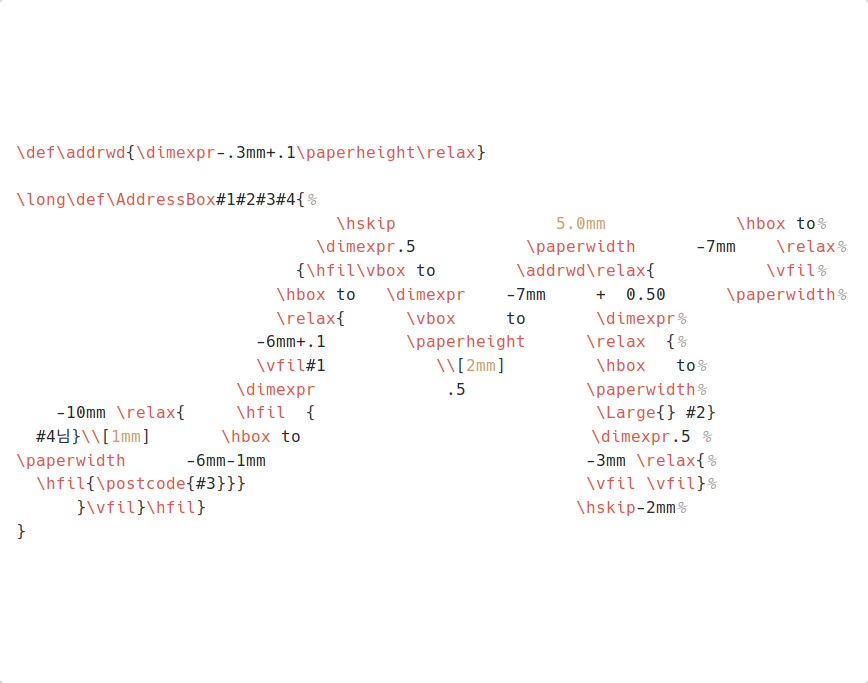
\includegraphics[width=0.5\textwidth]{msquare}
    \caption{Gorgeous}
  \end{center}
\end{figure}
  \end{minted}
\end{frame}

\begin{frame}[fragile]
  \frametitle{\texttt{tabular}}
  \framesubtitle{예시만 넣어 놓으면 택님께서 설명해 주실 거예요}
  \url{https://www.tablesgenerator.com/}
\end{frame}

\section{Macros\,/\,Definitions}

\begin{frame}[fragile]
  \frametitle{매크로}
  \framesubtitle{귀찮은 일은 싫어하는 사람들의 모임}
  \begin{itemize}
    \item<1-> 편집부장님: ``레이텍으로 구구단을 만들어 주세요!''
    \item<1-> 안타까운 사람들: \mintinline[escapeinside=||]{latex}{$2 \times 2 = 4$, $2 \times 3 = 6$, ...}
    \item<2-> 매크로를 배운 후:\vspace{-1em}
    \begin{minted}{latex}
\newcounter{left} \newcounter{right}
\forloop{left}{2}{\value{left} < 10}{%
  \noindent\forloop{right}{2}{\value{right} < 10}{%
    $\arabic{left} \times \arabic{right} =
      \the\numexpr\arabic{left} * \arabic{right}\relax$,
  }
  \par
}
    \end{minted}
  \end{itemize}
\end{frame}

\begin{frame}[fragile]
  \frametitle{기본적인 매크로}
  \framesubtitle{plain \TeX 버전}
  \begin{itemize}
    \item \mintinline[escapeinside=||]{latex}{\def\mymacro#1#2#3{\textit{#1}#2\textrm{#3}}}
    \begin{itemize}
      \item \mintinline[escapeinside=||]{latex}{\def} 매크로 정의를 시작하는 토큰
      \item \mintinline[escapeinside=||]{latex}{\mymacro#1#2#3} 매크로 이름과 parameter 개수 (<9), 즉 parameter를 \mintinline[escapeinside=||]{latex}{\mymacro{p1}{p2}{p3}}처럼 받는다는 이야기
      \item \mintinline[escapeinside=||]{latex}{{\textit{#1}#2\textrm{#3}}} 매크로 이름이 나온 후 처음으로 \texttt{\{}를 만나면 그 매크로를 전개했을 때 나오는 매크로의 `내용'을 정의하게 됩니다.
    \end{itemize}
    \item 다른 기호를 쓸 수도 있어요!! \mintinline[escapeinside=||]{latex}{\mymacro[#1]#2\middle #3{#1#2#3}} 패턴 매칭처럼 행동합니다. 이 방법은 plain \TeX에서 가끔 배열을 다뤄야 할 때 유용해요. 
    \item 한글은 쓰지 마세요...
  \end{itemize}
\end{frame}
\begin{frame}[fragile]
  \frametitle{기본적인 매크로}
  \framesubtitle{\LaTeXe 버전}
  \begin{itemize}
    \item \mintinline[escapeinside=||]{latex}{\newcommand{\mymacro}[3][A]{#1,#2,#3}} 
    \begin{itemize}
      \item \mintinline[escapeinside=||]{latex}{\newcommand} 매크로 정의를 시작하는 토큰
      \item \mintinline[escapeinside=||]{latex}{{\mymacro}} 매크로 이름
      \item \mintinline[escapeinside=||]{latex}{[3]} parameter 개수 (<9)
      \item \mintinline[escapeinside=||]{latex}{[A]} \texttt{\#1}의 기본값 (기본값은 가장 처음 인자 한 개까지만 지정 가능하며, 기본값이 있는 optional한 인자는 \texttt{\{...\}}가 아닌 \texttt{[...]}로 묶어주어야 합니다.)
    \end{itemize}
  \end{itemize}
\end{frame}
\begin{frame}[fragile]
  \frametitle{기본적인 매크로}
  \framesubtitle{\LaTeX\,3 버전}
  \begin{itemize}
    \item \mintinline[escapeinside=||]{latex}{\NewDocumentCommand{\mymacro}{s m o O{3}}{#1,#2,#3,#4}} 
    \begin{itemize}
      \item \mintinline[escapeinside=||]{latex}{\usepackage{xparse, expl3}} \LaTeX\,3 관련
      \item \mintinline[escapeinside=||]{latex}{\NewDocumentCommand} 매크로 정의를 시작하는 토큰
      \item \mintinline[escapeinside=||]{latex}{{\mymacro}} 매크로 이름
      \item \mintinline[escapeinside=||]{latex}{{s m o O{3}}} parameter 개수와 그 spec
      \begin{itemize}
        \item \texttt{m}: 필수 인자
        \item \texttt{o}: 기본값 없는 optional한 인자; 기본값 없는 optional 인자에 값이 주어지지 않으면 대신 \texttt{-NoValue-}라는 값이 들어갑니다.
        \item \texttt{O\{3\}}: 기본값이 3인 optional한 인자
        \item \texttt{s}: 별표가 있는지 없는지 감지
        \item 다른 spec은 패키지 \texttt{xparse} 매뉴얼 참조
      \end{itemize}
    \end{itemize}
    \item 지금까지 나온 매크로들은 텍스트와 수식 모드 모두에서 쓸 수 있습니다.
  \end{itemize}
\end{frame}

\begin{frame}[fragile]
  \frametitle{매크로 예시!!}
  \framesubtitle{간단하고 쉬운 것}
  \begin{itemize}
    \item $\boldsymbol{\alpha}$를 간단하게 쓰고 싶을 때:
    \item \mintinline[escapeinside=||]{latex}{\newcommand{\bsalpha}{\boldsymbol{\alpha}}} \newcommand{\bsalpha}{$\boldsymbol{\alpha}$} \bsalpha
    \item $\mathbb Z$를 간단하게 쓰고 싶을 때:
    \item \mintinline[escapeinside=||]{latex}{\newcommand{\ZZ}{\mathbb{Z}}} \newcommand{\ZZ}{{\mathbb Z}} $\ZZ$
  \end{itemize}
\end{frame}

\begin{frame}[fragile]
  \frametitle{매크로 예시!!}
  \framesubtitle{간단하고 쉬운 것}
  \begin{itemize}
    \item 벡터 표기하기
    \begin{itemize}
      \item \mintinline[escapeinside=||]{latex}{$\vecNotation{X}$}를 하면 $(X_1, X_2, X_3)^{\mathsf{T}}$가 나오게 하고 싶다!
      \item \mintinline[escapeinside=||]{latex}{$\vecNotation{X}[1]$}를 하면 $(X_1)$가 나오게 하고 싶다!
      \item \mintinline[escapeinside=||]{latex}{$\vecNotation{X}[2]$}를 하면 $(X_1, X_2)^{\mathsf{T}}$가 나오게 하고 싶다!
      \item \mintinline[escapeinside=||]{latex}{$\vecNotation{X}[4]$}를 하면 $(X_1, X_2,\dots,X_4)^{\mathsf{T}}$가 나오게 하고 싶다!
      \item \mintinline[escapeinside=||]{latex}{$\vecNotation{X}[n]$}를 하면 $(X_1, X_2,\dots,X_n)^{\mathsf{T}}$가 나오게 하고 싶다!
    \end{itemize}
  \end{itemize}
\end{frame}

\setstretch{0.9}
\begin{frame}[fragile]
  \frametitle{매크로 예시!!}
  \framesubtitle{간단하고 쉬운 것}
  \vspace*{-2em}
  \begin{minted}[fontsize=\footnotesize]{latex}
\ExplSyntaxOn % _와 :를 매크로 이름에 쓸 수 있게 만듭니다.
\NewDocumentCommand{\vecNotation}{m O{3}}{
  % \tl_if_eq:nnTF{토큰 리스트1}{토큰 리스트2}{같을 때}{다를 때}
  \tl_if_eq:nnTF{#2}{1}{
    (#1\sb 1) % \ExplSyntaxOn이 _를 문자로 바꾸므로 
              % \sb라는 명령어로 subscript를 만듭니다.
  }{
    \tl_if_eq:nnTF{#2}{2}{
      (#1\sb 1, #1\sb 2)^{\mathsf{T}}
    }{
      \tl_if_eq:nnTF{#2}{3}{
        (#1\sb 1, #1\sb 2, #1\sb 3)^{\mathsf{T}}
      }{
        (#1\sb 1, #1\sb 2, \dots, #1\sb{#2})^{\mathsf{T}}
      }
    }
  }
}
\ExplSyntaxOff % _와 :를 다시 각자의 목적으로 되돌립니다.
  \end{minted}
\end{frame}
\setstretch{1.3}


\begin{frame}[fragile]
  \frametitle{Counter}
  \framesubtitle{For \LaTeXe}
  \begin{itemize}
    \item 정수(integer)형 변수 역할
    \item \mintinline{latex}{\newcounter{CounterName}} 새 카운터를 만듭니다.
    \item \mintinline{latex}{\setcounter{CounterName}{value}} 카운터 값 지정
    \item \mintinline{latex}{\addtocounter{CounterName}{value}} 카운터에 값을 더하기 (음수도 가능)
    \item \mintinline{latex}{\value{CounterName}} 카운터 값 출력
  \end{itemize}
\end{frame}




\begin{frame}[fragile]
  \frametitle{For loop}
  \framesubtitle{\texttt{forloop}, \texttt{pgffor}}
  \begin{itemize}
    \item \mintinline{latex}{\forloop[step]{counter}{initial}{condition}{code}}
    \begin{itemize}
      \item \mintinline{latex}{\usepackage{forloop}}
      \item \mintinline{latex}{\newcounter{ct}}
      \item[] \mintinline{latex}{\forloop{ct}{1}{\value{ct} < 10}{\arabic{ct} }}
      \item 1 2 3 4 5 6 7 8 9\textvisiblespace
    \end{itemize}
    \item \mintinline{latex}{\foreach \macro in {1,4,...,10}{...}}
    \begin{itemize}
      \item \mintinline{latex}{\usepackage{pgffor}}
    \setstretch{1.1}
    \item[\mysymboli\;] \vspace{-1.5em}\begin{minted}[fontsize=\footnotesize]{latex}
\newcommand{\repsum}[3]{%
  \foreach \i in {1,...,#1}{
    \ifnum\i>1
      + #2_{\i} #3_{\i}
    \else
      #2_{\i} #3_{\i}
    \fi
  }
}
      \end{minted}
    \setstretch{1.3}
  \end{itemize}
  \end{itemize}
\end{frame}


\begin{frame}[fragile]
  \frametitle{커버하지 않은 내용}
  \framesubtitle{너무 많아요}
  \texttt{\char`\\label\char`\\ref\char`\\url\char`\\definecolor\char`\\textcolor\char`\\color\char`\\newenvironment\\\char`\\expandafter\char`\\noexpand\char`\\IfNoValueTF\char`\\IfBooleanTF\char`\\makeatletter\\\char`\\makeatother\char`\\@author\char`\\@date\char`\\begin\{tikz\}...\char`\\end\{tikz\}\char`\\edef\\\char`\\@gobble\char`\\relax\char`\\dimexpr\char`\\numexpr
  \char`\\the\char`\\meaning\char`\\global\\\char`\\xdef\char`\\csname...\char`\\endcsname\char`\\@firstofone\char`\\z@\char`\\@car\char`\\@cdr\char`\\@nil\\\char`\\toks@\char`\\loop\char`\\@for\char`\\g@addto@macro\char`\\parskip\char`\\parindent\char`\\protected\\ \char`\\unexpanded\char`\\renewcommand\char`\\RedeclareSectionCommand\char`\\hbox\char`\\pbox\\\char`\\rule\char`\\raisebox\char`\\kern\char`\\hskip\char`\\vskip\char`\\glueexpr\char`\\allowdisplaybreaks,...}

  \vspace{1em}
  패키지: \texttt{expl3}, \texttt{xkeyval}, \texttt{pgf}, \texttt{tikz}, \texttt{tikzcd}, \texttt{ulem}, \texttt{tcolorbox}, \texttt{bibtex}, \texttt{natbib}, \texttt{fancyhdr}, \texttt{tcolorbox}, \texttt{environ}, \texttt{listings}, \texttt{minted}, \texttt{beamer, \dots}

  \vspace{1em} 다른 언어의 도움: \LuaLaTeX, HaTeX, PyTeX, \dots
\end{frame}

\section{\texttt{MathLetter.sty}}
\setstretch{1.1}
\begin{frame}[fragile]
  \frametitle{\texttt{MathLetter.sty}}
  \framesubtitle{디자인을 하나하나 만들고 있기는 힘드니까...}
  \begin{itemize}
    \item \url{https://github.com/msquare-kaist/mathletter-package}
    \item 매뉴얼: \url{https://github.com/msquare-kaist/mathletter-package/blob/master/documents/manual.pdf}
    \item 매뉴얼에 안 쓰여 있는 것: \texttt{\char`\\PrintBibliography}와 \texttt{\char`\\Footnote}
    \begin{itemize}
    \item \texttt{\char`\\PrintBibliography}: .tex 파일 상단 \mintinline{latex}{\documentclass, \usepackage} 밑에 참고문헌 .bib 파일을 추가하고 (\mintinline{latex}{\addbibresource{filename.bib}}) \mintinline{latex}{\end{document}} 전에 \mintinline{latex}{\PrintBibliography}를 입력하면 참고문헌이 나옵니다. (컴파일은 두 번 해야합니다.)
    \item \texttt{\char`\\Footnote}: 그냥 \mintinline{latex}{\footnote}와 사용법은 같습니다. 여러 environment 안에 각주가 갇히는 현상을 방지하기 위한 매크로입니다.
    \end{itemize}
    \item \texttt{\char`\\MSquare}: \mintinline{latex}{\MSquare[1/2], \MSquare, \MSquare[2]}
    \begin{itemize}
    \item  \MSquare[1/2], \MSquare, \MSquare[2]
    \item 아직 소수는 입력이 안 되는데 언젠간 누군가 고칠 예정입니다.
    \end{itemize}
  \end{itemize}
\end{frame}

\section{끝}

\end{document}

% \mintinline[escapeinside=||]{latex}{\textit{italic}}